\section{Introduction}
\label{sec:intro}

Supporting sequences (arrays) with efficient (constant time) random
access updates has been a persistent problem in functional languages
(pun intended).  It is easy to implement such sequences with constant
time random access reads (using arrays stored as contiguous memory),
or to implement with logarithmic time reads and updates using balanced
trees, but getting both in constant time cannot be done without some
form of extension.
%~\cite{Pippenger97}.  
This means that algorithms
for many fundamental problems are a logarithmic factor slower in
functional languages than in imperative languages.  This includes
algorithms for basic problems such as generating a random permutation,
and for many important graph problems (e.g.,
shortest-unweighted-paths, connected components, biconnected
components, topological sort, and cycle detection).  Simple algorithms
for these problems take linear time in the imperative setting, but an
additional logarithmic factor in time in the functional setting, at
least without extensions.

A variety of approaches have been suggested to alleviate this problem.
Many of the approaches are based on the observation that if there is
only a single reference to an array, it can be safely updated in
place.  The most common such approach is to use
monads~\cite{Moggi89,Wadler95}.  Monads can force code to be single
threaded and can thread mutable arrays (or other mutable
state) implicitly so the only reference to them is the current one.
Haskell supplies the ST monad for this purpose.  King and Launchbery,
for example, use STMonads with an array to implement depth first (DFS)
search in linear work~\cite{KL95}.  Guzman and Hudak's single-threaded
lambda calculus also uses the idea of single threading the
computation~\cite{GH90}, and motivate the approach based on allowing
for fast array updates.  The problem with using these approaches is
that it is basically implementing a second imperative language within
a functional language.  Using monads means using a new syntax not just
for the operations themselves but for everything the operations are
embedded in.  Indeed King and Launchbery have to write completely
different code for DFS, even though it is only for efficiency and not
correctness (it is trivial to implement DFS in $O(m \log n)$ time
purely functionally).  Monads also do not allow keeping persistent
versions of structures, exactly because the state can be changed.
More importantly, however, it forces the program itself to be single
threaded, inhibiting parallelism.

A second approach is to use a type system that enforces the
single-threadedness of individual arrays rather than the program as a
whole.  This can be done with linear types~\cite{Girard87,Wadler90},
which can be used to ensure that references are not duplicated.  This
is more flexible than monads, since it allows the threading of the
data to be distinct from the threading of the program.  However, such
type systems are not available in most languages, and they can be hard
to reason about.

A third approach is to support fully functional arrays in a general
functional language, and to check in the program if they happen to be
used in a single threaded manner.  This can be done, for example, by
using reference counting~\cite{HB85,Hudak86}.  The idea is to keep
track of how many references there are to an array and update inplace
if there is only one.  Hudak describes techniques to statically
analyze code to determine that at certain points in the code a count
must be one, and therefore it is safe to replace an update with an
inplace update.  The problem with this approach is that the efficiency
of the code depends heavily on the effectiveness of the compiler and
the specific way the code is written, and it can therefore be hard for
the user to reason about efficiency.

The last approach is to fully support functional arrays, even with
sharing, but more efficiently than as a simple array or tree.  This is
sometimes referred to as version tree arrays~\cite{AHN88} or fully
persistent arrays~\cite{DSST89}.  The idea is to maintain a version
tree for an array (or more generally other data types), such that any
node of the tree can be updated to create a new leaf below it with the
modified value, without effecting the value of other nodes.  Dietz
showed that arrays can be maintained fully persistently using
$O(\log\log n)$ time per operation (read or write).  Holmstrom, Hughes
and others (see \cite{AHN88}) suggested storing a version tree by
keeping the full array at the root, and a each node represents an
update.  Chuang's approach ~\cite{chuang} supports $O(1)$ accesses and
insertions to the most recent version of arrays, however accessing old
versions of the array takes $O(n)$ work which is often impractical.
O'Neill and Warren~\cite{oneill} describe various improvements.
The problem with these approaches is that they can be very complicated,
and only efficient in certain cases.   Furthermore it can be hard to
reason about the performance.

None of the existing approaches support concurrent operations on
arrays.  O' Neill suggests (in passing) having a lock for each element
of the array. However, when many threads contend for the same element,
this would serialize accesses and make accesses not
$O(1)$. Additionally, per-element locks add significant memory
overhead.  
% Separation logic ~\cite{reynolds} could be used to
% parallelize divide and conquer algorithms on arrays however they would
% severely restrict the way functional arrays can be used.

\subsection*{Our Approach}

In this paper we present an approach for efficiently supporting
functional arrays.  It uses some ideas from the previous approaches
but unlike the previous approaches it supplies a well
defined cost semantics, and supports parallelism, and without language
extensions.  More specifically the approach has the
following important features.
\begin{enumerate}
\item It has fully functional value semantics (dynamic
  semantics)---i.e., when not considering costs, arrays act no
  differently than purely functional arrays.
\item It requires no changes in existing languages and no special
  types, syntactic extensions, etc.  Programs can be efficient---i.e.,
  constant time reads and writes---when using a completely standard
  functional programming style.
\item The approach supports nested parallelism---arrays can be passed
  to parallel calls and safely updated and read, again with a purely
  functional semantics.
\item We supply a well defined cost semantics, which can be used to
  formally analyze the cost of any program.  The semantics captures
  both sequential and parallel costs.
\item We describe a cost-bounded implementation which maps costs in the
  model to costs on either a sequential or parallel RAM (PRAM).
\item
Although accessing old versions of an array is more expensive than
accessing new versions (as defined in the cost semantics), reading old
versions never costs more than $O(\log n)$ work.
\end{enumerate}
We have implemented the approach and in this paper present some
performance numbers.

Although our value semantics are purely functional (and compositional)
our cost semantics are not---they require passing a store and modeling
costs based on the order the store is threaded.  The reader might
object to this non-functional nature of the cost semantics, but we
note that non-functional costs are also requires in call-by-need
(lazy) languages, which supply a functional value semantics but an
imperative cost semantics.  In fact from the value point of view,
call-by-need is no different from call-by-name, and it is only when
considering costs that they differ.  The cost semantics of
call-by-need~\cite{AMOFW95} is completely non-functional
(non-compositional).  Furthermore it is likely significantly more
complicated to reason about than the cost semantics we present in this
paper.

\begin{figure}[!ht]
\centering 
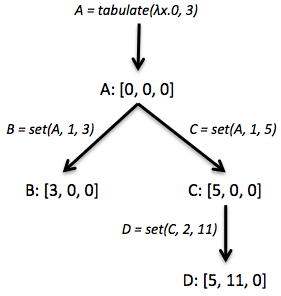
\includegraphics[scale=0.45]{leaf_interior_intro}
\nocaptionrule \caption{Example usage of functional arrays}
\label{fig:leaf_interior_intro}
\end{figure}

In this paper we consider arrays with three functions: \tabulate{},
\get{} (read), and \set{} (write).  As usual, \tabulate{}$(f,n)$
creates a new array of length $n$ by applying the function $f$ to
$[0, \ldots, n-1]$, \get$(A,i)$ returns the $i^{th}$ element of $A$, and
\set$(A,i,v)$ sets the $i^{th}$ element of $A$ to $v$ returning a
``new'' array (in the following discussion $n$ refers to the length of
an array).  Figure~\ref{fig:leaf_interior_intro} gives an example.  As
in previous work~\cite{AHN88} the history of an array after it is
created with \tabulate{} can be viewed as a version tree.  A version
tree has interior nodes and leaves.  In the figure, after all
functions are applied, arrays $A$ and $C$ are \emph{interior nodes},
and arrays $B$ and $D$ are \emph{leaves} of the version tree.  In our
cost semantics applying \get{} and \set{} to arrays at the leafs takes
constant work, but applying them to interior nodes is more expensive.
We define a cost semantics that identifies whether an array is a leaf
or interior node and charges for the cost of \get{} and \set{}
appropriately.  This requires threading a store that maps labels
(corresponding to each array) to indicate whether the array is a leaf
or interior.

Since we are also interested in parallelism, we include fork-join
parallelism in our language and semantics.    Our cost semantics then
models the cost of arrays when used in parallel.  This is non-trivial
since parallel tasks can read and update an array in parallel.
To deal with this, we compute the work of each forked task separately,
and then charge additional work at the join point if an array is used
in both forks.

To implement our functional arrays, we maintain at each leaf of the
version tree an array of the most recent values.  We also keep with
each location a change-log that keeps track of values at interior
nodes of the version tree.  Applying \get{} to a leaf only requires a
lookup in the array.  Applying \set{} to a leaf only requires updating
the array, and adding an element to the change log for the old
version.  Applying \get{} to an interior nodes requires a binary
search on the change log, which can be bounded by $O(\log n)$ time.
To ensure that change logs do not get too large, whenever the total
size across all change logs reaches $n$, the array is copied.   This
requires $O(n)$ time, but can be amortized against the updates.
Applying \set{} to an interior node requires creating a new array,
and copying values to it.   This requires $O(n)$ time.    

We give a wait-free concurrent implementation that uses careful
synchronization. We prove linearizability of the implementation and
use that to prove that our arrays work correctly when used
concurrently. Finally, we give a provable implementation for our cost
dynamics.
